\documentclass[1p]{elsarticle_modified}
%\bibliographystyle{elsarticle-num}

%\usepackage[colorlinks]{hyperref}
%\usepackage{abbrmath_seonhwa} %\Abb, \Ascr, \Acal ,\Abf, \Afrak
\usepackage{amsfonts}
\usepackage{amssymb}
\usepackage{amsmath}
\usepackage{amsthm}
\usepackage{scalefnt}
\usepackage{amsbsy}
\usepackage{kotex}
\usepackage{caption}
\usepackage{subfig}
\usepackage{color}
\usepackage{graphicx}
\usepackage{xcolor} %% white, black, red, green, blue, cyan, magenta, yellow
\usepackage{float}
\usepackage{setspace}
\usepackage{hyperref}

\usepackage{tikz}
\usetikzlibrary{arrows}

\usepackage{multirow}
\usepackage{array} % fixed length table
\usepackage{hhline}

%%%%%%%%%%%%%%%%%%%%%
\makeatletter
\renewcommand*\env@matrix[1][\arraystretch]{%
	\edef\arraystretch{#1}%
	\hskip -\arraycolsep
	\let\@ifnextchar\new@ifnextchar
	\array{*\c@MaxMatrixCols c}}
\makeatother %https://tex.stackexchange.com/questions/14071/how-can-i-increase-the-line-spacing-in-a-matrix
%%%%%%%%%%%%%%%

\usepackage[normalem]{ulem}

\newcommand{\msout}[1]{\ifmmode\text{\sout{\ensuremath{#1}}}\else\sout{#1}\fi}
%SOURCE: \msout is \stkout macro in https://tex.stackexchange.com/questions/20609/strikeout-in-math-mode

\newcommand{\cancel}[1]{
	\ifmmode
	{\color{red}\msout{#1}}
	\else
	{\color{red}\sout{#1}}
	\fi
}

\newcommand{\add}[1]{
	{\color{blue}\uwave{#1}}
}

\newcommand{\replace}[2]{
	\ifmmode
	{\color{red}\msout{#1}}{\color{blue}\uwave{#2}}
	\else
	{\color{red}\sout{#1}}{\color{blue}\uwave{#2}}
	\fi
}

\newcommand{\Sol}{\mathcal{S}} %segment
\newcommand{\D}{D} %diagram
\newcommand{\A}{\mathcal{A}} %arc


%%%%%%%%%%%%%%%%%%%%%%%%%%%%%5 test

\def\sl{\operatorname{\textup{SL}}(2,\Cbb)}
\def\psl{\operatorname{\textup{PSL}}(2,\Cbb)}
\def\quan{\mkern 1mu \triangleright \mkern 1mu}

\theoremstyle{definition}
\newtheorem{thm}{Theorem}[section]
\newtheorem{prop}[thm]{Proposition}
\newtheorem{lem}[thm]{Lemma}
\newtheorem{ques}[thm]{Question}
\newtheorem{cor}[thm]{Corollary}
\newtheorem{defn}[thm]{Definition}
\newtheorem{exam}[thm]{Example}
\newtheorem{rmk}[thm]{Remark}
\newtheorem{alg}[thm]{Algorithm}

\newcommand{\I}{\sqrt{-1}}
\begin{document}

%\begin{frontmatter}
%
%\title{Boundary parabolic representations of knots up to 8 crossings}
%
%%% Group authors per affiliation:
%\author{Yunhi Cho} 
%\address{Department of Mathematics, University of Seoul, Seoul, Korea}
%\ead{yhcho@uos.ac.kr}
%
%
%\author{Seonhwa Kim} %\fnref{s_kim}}
%\address{Center for Geometry and Physics, Institute for Basic Science, Pohang, 37673, Korea}
%\ead{ryeona17@ibs.re.kr}
%
%\author{Hyuk Kim}
%\address{Department of Mathematical Sciences, Seoul National University, Seoul 08826, Korea}
%\ead{hyukkim@snu.ac.kr}
%
%\author{Seokbeom Yoon}
%\address{Department of Mathematical Sciences, Seoul National University, Seoul, 08826,  Korea}
%\ead{sbyoon15@snu.ac.kr}
%
%\begin{abstract}
%We find all boundary parabolic representation of knots up to 8 crossings.
%
%\end{abstract}
%\begin{keyword}
%    \MSC[2010] 57M25 
%\end{keyword}
%
%\end{frontmatter}

%\linenumbers
%\tableofcontents
%
\newcommand\colored[1]{\textcolor{white}{\rule[-0.35ex]{0.8em}{1.4ex}}\kern-0.8em\color{red} #1}%
%\newcommand\colored[1]{\textcolor{white}{ #1}\kern-2.17ex	\textcolor{white}{ #1}\kern-1.81ex	\textcolor{white}{ #1}\kern-2.15ex\color{red}#1	}

{\Large $\underline{12n_{0769}~(K12n_{0769})}$}

\setlength{\tabcolsep}{10pt}
\renewcommand{\arraystretch}{1.6}
\vspace{1cm}\begin{tabular}{m{100pt}>{\centering\arraybackslash}m{274pt}}
\multirow{5}{120pt}{
	\centering
	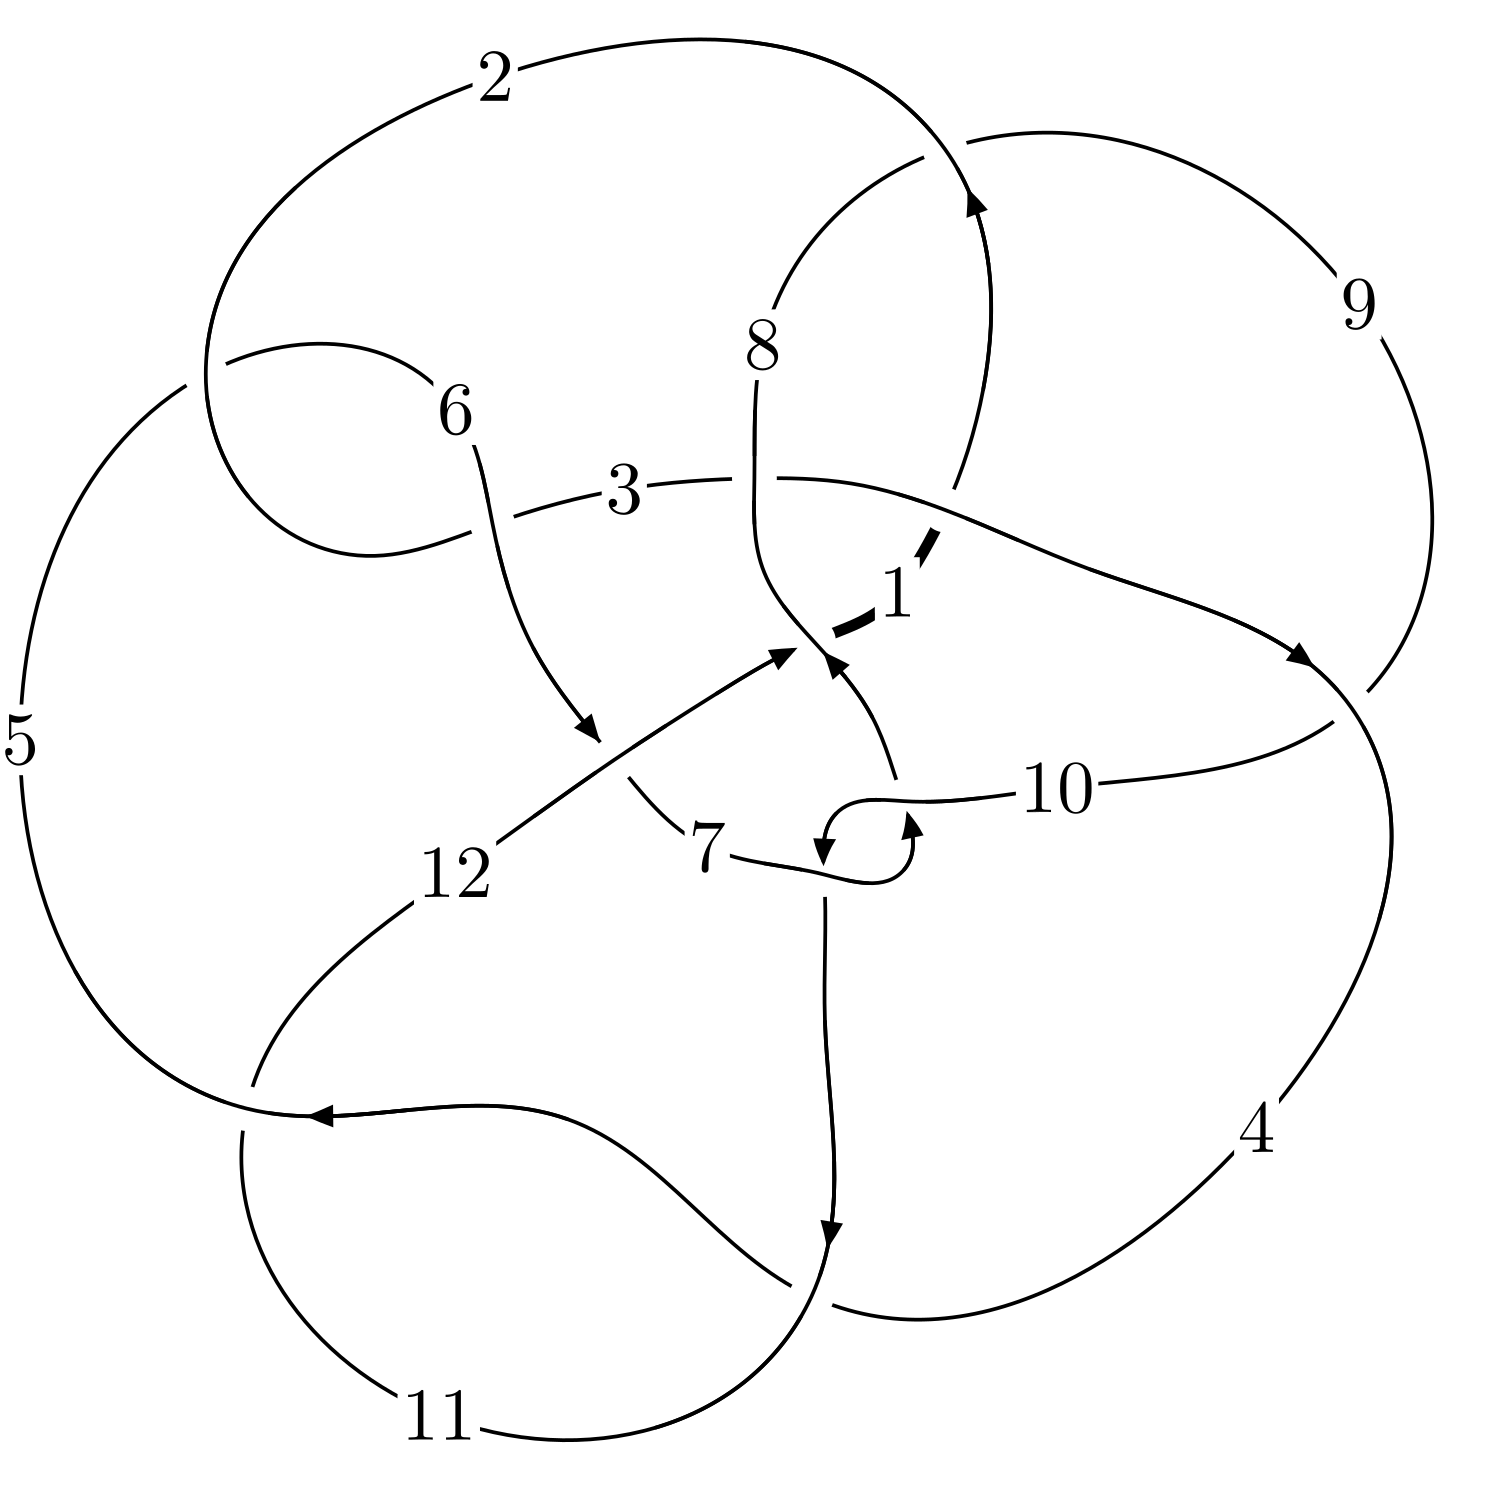
\includegraphics[width=112pt]{../../../GIT/diagram.site/Diagrams/png/2858_12n_0769.png}\\
\ \ \ A knot diagram\footnotemark}&
\allowdisplaybreaks
\textbf{Linearized knot diagam} \\
\cline{2-2}
 &
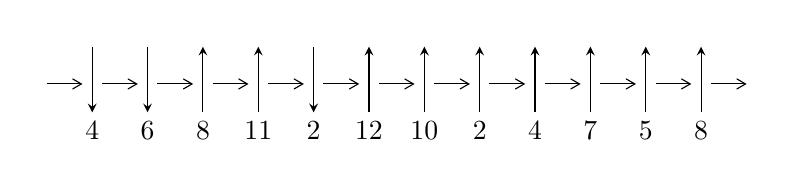
\begin{tikzpicture}[x=20pt, y=17pt]
	% nodes
	\node (C0) at (0, 0) {};
	\node (C1) at (1, 0) {};
	\node (C1U) at (1, +1) {};
	\node (C1D) at (1, -1) {4};

	\node (C2) at (2, 0) {};
	\node (C2U) at (2, +1) {};
	\node (C2D) at (2, -1) {6};

	\node (C3) at (3, 0) {};
	\node (C3U) at (3, +1) {};
	\node (C3D) at (3, -1) {8};

	\node (C4) at (4, 0) {};
	\node (C4U) at (4, +1) {};
	\node (C4D) at (4, -1) {11};

	\node (C5) at (5, 0) {};
	\node (C5U) at (5, +1) {};
	\node (C5D) at (5, -1) {2};

	\node (C6) at (6, 0) {};
	\node (C6U) at (6, +1) {};
	\node (C6D) at (6, -1) {12};

	\node (C7) at (7, 0) {};
	\node (C7U) at (7, +1) {};
	\node (C7D) at (7, -1) {10};

	\node (C8) at (8, 0) {};
	\node (C8U) at (8, +1) {};
	\node (C8D) at (8, -1) {2};

	\node (C9) at (9, 0) {};
	\node (C9U) at (9, +1) {};
	\node (C9D) at (9, -1) {4};

	\node (C10) at (10, 0) {};
	\node (C10U) at (10, +1) {};
	\node (C10D) at (10, -1) {7};

	\node (C11) at (11, 0) {};
	\node (C11U) at (11, +1) {};
	\node (C11D) at (11, -1) {5};

	\node (C12) at (12, 0) {};
	\node (C12U) at (12, +1) {};
	\node (C12D) at (12, -1) {8};
	\node (C13) at (13, 0) {};

	% arrows
	\draw[->,>={angle 60}]
	(C0) edge (C1) (C1) edge (C2) (C2) edge (C3) (C3) edge (C4) (C4) edge (C5) (C5) edge (C6) (C6) edge (C7) (C7) edge (C8) (C8) edge (C9) (C9) edge (C10) (C10) edge (C11) (C11) edge (C12) (C12) edge (C13) ;	\draw[->,>=stealth]
	(C1U) edge (C1D) (C2U) edge (C2D) (C3D) edge (C3U) (C4D) edge (C4U) (C5U) edge (C5D) (C6D) edge (C6U) (C7D) edge (C7U) (C8D) edge (C8U) (C9D) edge (C9U) (C10D) edge (C10U) (C11D) edge (C11U) (C12D) edge (C12U) ;
	\end{tikzpicture} \\
\hhline{~~} \\& 
\textbf{Solving Sequence} \\ \cline{2-2} 
 &
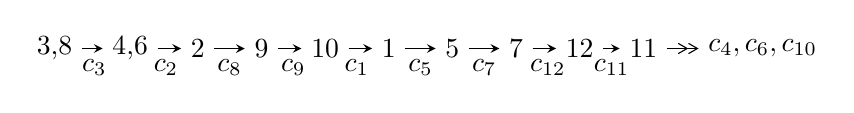
\begin{tikzpicture}[x=23pt, y=7pt]
	% node
	\node (A0) at (-1/8, 0) {3,8};
	\node (A1) at (17/16, 0) {4,6};
	\node (A2) at (17/8, 0) {2};
	\node (A3) at (25/8, 0) {9};
	\node (A4) at (33/8, 0) {10};
	\node (A5) at (41/8, 0) {1};
	\node (A6) at (49/8, 0) {5};
	\node (A7) at (57/8, 0) {7};
	\node (A8) at (65/8, 0) {12};
	\node (A9) at (73/8, 0) {11};
	\node (C1) at (1/2, -1) {$c_{3}$};
	\node (C2) at (13/8, -1) {$c_{2}$};
	\node (C3) at (21/8, -1) {$c_{8}$};
	\node (C4) at (29/8, -1) {$c_{9}$};
	\node (C5) at (37/8, -1) {$c_{1}$};
	\node (C6) at (45/8, -1) {$c_{5}$};
	\node (C7) at (53/8, -1) {$c_{7}$};
	\node (C8) at (61/8, -1) {$c_{12}$};
	\node (C9) at (69/8, -1) {$c_{11}$};
	\node (A10) at (11, 0) {$c_{4},c_{6},c_{10}$};

	% edge
	\draw[->,>=stealth]	
	(A0) edge (A1) (A1) edge (A2) (A2) edge (A3) (A3) edge (A4) (A4) edge (A5) (A5) edge (A6) (A6) edge (A7) (A7) edge (A8) (A8) edge (A9) ;
	\draw[->>,>={angle 60}]	
	(A9) edge (A10);
\end{tikzpicture} \\ 

\end{tabular} \\

\footnotetext{
The image of knot diagram is generated by the software ``\textbf{Draw programme}" developed by Andrew Bartholomew(\url{http://www.layer8.co.uk/maths/draw/index.htm\#Running-draw}), where we modified some parts for our purpose(\url{https://github.com/CATsTAILs/LinksPainter}).
}\phantom \\ \newline 
\centering \textbf{Ideals for irreducible components\footnotemark of $X_{\text{par}}$} 
 
\begin{align*}
I^u_{1}&=\langle 
3.83864\times10^{337} u^{65}-1.18349\times10^{338} u^{64}+\cdots+1.06451\times10^{342} b-1.02256\times10^{342},\\
\phantom{I^u_{1}}&\phantom{= \langle  }-1.56678\times10^{341} u^{65}+4.83301\times10^{341} u^{64}+\cdots+1.39504\times10^{345} a-4.89344\times10^{345},\\
\phantom{I^u_{1}}&\phantom{= \langle  }u^{66}-3 u^{65}+\cdots+1022 u-2621\rangle \\
I^u_{2}&=\langle 
-5.16198\times10^{14} u^{22}+4.96659\times10^{15} u^{21}+\cdots+6.69596\times10^{15} b-5.25349\times10^{15},\\
\phantom{I^u_{2}}&\phantom{= \langle  }-1.04392\times10^{16} u^{22}+4.70651\times10^{16} u^{21}+\cdots+6.69596\times10^{15} a+1.86768\times10^{16},\;u^{23}-4 u^{22}+\cdots-2 u-1\rangle \\
\\
\end{align*}
\raggedright * 2 irreducible components of $\dim_{\mathbb{C}}=0$, with total 89 representations.\\
\footnotetext{All coefficients of polynomials are rational numbers. But the coefficients are sometimes approximated in decimal forms when there is not enough margin.}
\newpage
\renewcommand{\arraystretch}{1}
\centering \section*{I. $I^u_{1}= \langle 3.84\times10^{337} u^{65}-1.18\times10^{338} u^{64}+\cdots+1.06\times10^{342} b-1.02\times10^{342},\;-1.57\times10^{341} u^{65}+4.83\times10^{341} u^{64}+\cdots+1.40\times10^{345} a-4.89\times10^{345},\;u^{66}-3 u^{65}+\cdots+1022 u-2621 \rangle$}
\flushleft \textbf{(i) Arc colorings}\\
\begin{tabular}{m{7pt} m{180pt} m{7pt} m{180pt} }
\flushright $a_{3}=$&$\begin{pmatrix}1\\0\end{pmatrix}$ \\
\flushright $a_{8}=$&$\begin{pmatrix}0\\u\end{pmatrix}$ \\
\flushright $a_{4}=$&$\begin{pmatrix}1\\- u^2\end{pmatrix}$ \\
\flushright $a_{6}=$&$\begin{pmatrix}0.000112311 u^{65}-0.000346443 u^{64}+\cdots-0.270457 u+3.50774\\-0.0000360602 u^{65}+0.000111177 u^{64}+\cdots+0.748848 u+0.960593\end{pmatrix}$ \\
\flushright $a_{2}=$&$\begin{pmatrix}-0.0000377394 u^{65}+0.000109948 u^{64}+\cdots-0.553697 u-3.17735\\0.0000688159 u^{65}-0.000214201 u^{64}+\cdots-1.70637 u-0.657455\end{pmatrix}$ \\
\flushright $a_{9}=$&$\begin{pmatrix}0.0000148168 u^{65}-0.0000484765 u^{64}+\cdots+10.6401 u+0.738371\\0.0000284980 u^{65}-0.0000667785 u^{64}+\cdots+3.25127 u-0.315788\end{pmatrix}$ \\
\flushright $a_{10}=$&$\begin{pmatrix}0.0000381472 u^{65}-0.000101304 u^{64}+\cdots+13.9343 u+0.412030\\0.0000323377 u^{65}-0.0000782973 u^{64}+\cdots+3.20767 u-0.360774\end{pmatrix}$ \\
\flushright $a_{1}=$&$\begin{pmatrix}0.0000305409 u^{65}-0.000101770 u^{64}+\cdots-2.35564 u-3.84338\\0.0000751505 u^{65}-0.000234189 u^{64}+\cdots-1.89236 u-0.639428\end{pmatrix}$ \\
\flushright $a_{5}=$&$\begin{pmatrix}0.000151268 u^{65}-0.000479153 u^{64}+\cdots-2.21265 u+0.437691\\0.0000458801 u^{65}-0.000147106 u^{64}+\cdots-1.73849 u+0.898946\end{pmatrix}$ \\
\flushright $a_{7}=$&$\begin{pmatrix}0.000249270 u^{65}-0.000703271 u^{64}+\cdots-2.14183 u-0.415613\\0.0000538303 u^{65}-0.000153736 u^{64}+\cdots-0.578342 u-0.793468\end{pmatrix}$ \\
\flushright $a_{12}=$&$\begin{pmatrix}0.0000305409 u^{65}-0.000101770 u^{64}+\cdots-2.35564 u-3.84338\\0.0000682803 u^{65}-0.000211719 u^{64}+\cdots-1.80195 u-0.666025\end{pmatrix}$ \\
\flushright $a_{11}=$&$\begin{pmatrix}-0.000148371 u^{65}+0.000457620 u^{64}+\cdots+1.01930 u-2.54715\\-0.0000173746 u^{65}+0.0000555578 u^{64}+\cdots+0.940765 u-1.04993\end{pmatrix}$\\&\end{tabular}
\flushleft \textbf{(ii) Obstruction class $= -1$}\\~\\
\flushleft \textbf{(iii) Cusp Shapes $= -0.000277598 u^{65}+0.000900711 u^{64}+\cdots+12.6909 u+2.52964$}\\~\\
\newpage\renewcommand{\arraystretch}{1}
\flushleft \textbf{(iv) u-Polynomials at the component}\newline \\
\begin{tabular}{m{50pt}|m{274pt}}
Crossings & \hspace{64pt}u-Polynomials at each crossing \\
\hline $$\begin{aligned}c_{1}\end{aligned}$$&$\begin{aligned}
&u^{66}-4 u^{65}+\cdots+251 u+131
\end{aligned}$\\
\hline $$\begin{aligned}c_{2},c_{5}\end{aligned}$$&$\begin{aligned}
&u^{66}+2 u^{65}+\cdots-21 u+1
\end{aligned}$\\
\hline $$\begin{aligned}c_{3}\end{aligned}$$&$\begin{aligned}
&u^{66}-3 u^{65}+\cdots+1022 u-2621
\end{aligned}$\\
\hline $$\begin{aligned}c_{4},c_{11}\end{aligned}$$&$\begin{aligned}
&u^{66}+5 u^{65}+\cdots-402 u-171
\end{aligned}$\\
\hline $$\begin{aligned}c_{6}\end{aligned}$$&$\begin{aligned}
&u^{66}-2 u^{65}+\cdots-40871 u-2788
\end{aligned}$\\
\hline $$\begin{aligned}c_{7},c_{10}\end{aligned}$$&$\begin{aligned}
&u^{66}+6 u^{65}+\cdots+224 u+16
\end{aligned}$\\
\hline $$\begin{aligned}c_{8}\end{aligned}$$&$\begin{aligned}
&u^{66}+47 u^{64}+\cdots+18353 u-20690
\end{aligned}$\\
\hline $$\begin{aligned}c_{9}\end{aligned}$$&$\begin{aligned}
&u^{66}- u^{65}+\cdots+28988118 u-18025751
\end{aligned}$\\
\hline $$\begin{aligned}c_{12}\end{aligned}$$&$\begin{aligned}
&u^{66}-3 u^{65}+\cdots+418122130 u-132292613
\end{aligned}$\\
\hline
\end{tabular}\\~\\
\newpage\renewcommand{\arraystretch}{1}
\flushleft \textbf{(v) Riley Polynomials at the component}\newline \\
\begin{tabular}{m{50pt}|m{274pt}}
Crossings & \hspace{64pt}Riley Polynomials at each crossing \\
\hline $$\begin{aligned}c_{1}\end{aligned}$$&$\begin{aligned}
&y^{66}-94 y^{65}+\cdots-1810017 y+17161
\end{aligned}$\\
\hline $$\begin{aligned}c_{2},c_{5}\end{aligned}$$&$\begin{aligned}
&y^{66}-48 y^{65}+\cdots-193 y+1
\end{aligned}$\\
\hline $$\begin{aligned}c_{3}\end{aligned}$$&$\begin{aligned}
&y^{66}+83 y^{65}+\cdots+198203936 y+6869641
\end{aligned}$\\
\hline $$\begin{aligned}c_{4},c_{11}\end{aligned}$$&$\begin{aligned}
&y^{66}-29 y^{65}+\cdots-842526 y+29241
\end{aligned}$\\
\hline $$\begin{aligned}c_{6}\end{aligned}$$&$\begin{aligned}
&y^{66}+20 y^{65}+\cdots-290997577 y+7772944
\end{aligned}$\\
\hline $$\begin{aligned}c_{7},c_{10}\end{aligned}$$&$\begin{aligned}
&y^{66}+46 y^{65}+\cdots+58848 y^2+256
\end{aligned}$\\
\hline $$\begin{aligned}c_{8}\end{aligned}$$&$\begin{aligned}
&y^{66}+94 y^{65}+\cdots-15224156589 y+428076100
\end{aligned}$\\
\hline $$\begin{aligned}c_{9}\end{aligned}$$&$\begin{aligned}
&y^{66}+69 y^{65}+\cdots+2987872480868112 y+324927699114001
\end{aligned}$\\
\hline $$\begin{aligned}c_{12}\end{aligned}$$&$\begin{aligned}
&y^{66}+89 y^{65}+\cdots+205846697467622796 y+17501335454367769
\end{aligned}$\\
\hline
\end{tabular}\\~\\
\newpage\flushleft \textbf{(vi) Complex Volumes and Cusp Shapes}
$$\begin{array}{c|c|c}  
\text{Solutions to }I^u_{1}& \I (\text{vol} + \sqrt{-1}CS) & \text{Cusp shape}\\
 \hline 
\begin{aligned}
u &= \phantom{-}0.550266 + 0.896602 I \\
a &= -0.664287 - 1.148930 I \\
b &= -1.45948 - 0.16916 I\end{aligned}
 & -3.94389 - 6.56961 I & \phantom{-0.000000 } 0 \\ \hline\begin{aligned}
u &= \phantom{-}0.550266 - 0.896602 I \\
a &= -0.664287 + 1.148930 I \\
b &= -1.45948 + 0.16916 I\end{aligned}
 & -3.94389 + 6.56961 I & \phantom{-0.000000 } 0 \\ \hline\begin{aligned}
u &= -0.543655 + 0.904183 I \\
a &= -0.968879 - 0.052917 I \\
b &= -1.049230 - 0.220101 I\end{aligned}
 & -3.67929 + 0.01280 I & \phantom{-0.000000 } 0 \\ \hline\begin{aligned}
u &= -0.543655 - 0.904183 I \\
a &= -0.968879 + 0.052917 I \\
b &= -1.049230 + 0.220101 I\end{aligned}
 & -3.67929 - 0.01280 I & \phantom{-0.000000 } 0 \\ \hline\begin{aligned}
u &= \phantom{-}0.727225 + 0.435479 I \\
a &= \phantom{-}1.92650 - 1.46275 I \\
b &= \phantom{-}0.0406553 + 0.0835342 I\end{aligned}
 & \phantom{-}1.88021 + 5.73599 I & \phantom{-}12.0656 - 12.6009 I \\ \hline\begin{aligned}
u &= \phantom{-}0.727225 - 0.435479 I \\
a &= \phantom{-}1.92650 + 1.46275 I \\
b &= \phantom{-}0.0406553 - 0.0835342 I\end{aligned}
 & \phantom{-}1.88021 - 5.73599 I & \phantom{-}12.0656 + 12.6009 I \\ \hline\begin{aligned}
u &= -0.827890 + 0.059202 I \\
a &= \phantom{-}0.05599 - 1.88565 I \\
b &= \phantom{-}0.451189 + 1.104720 I\end{aligned}
 & \phantom{-}3.42513 - 3.10241 I & \phantom{-}9.91560 + 5.14976 I \\ \hline\begin{aligned}
u &= -0.827890 - 0.059202 I \\
a &= \phantom{-}0.05599 + 1.88565 I \\
b &= \phantom{-}0.451189 - 1.104720 I\end{aligned}
 & \phantom{-}3.42513 + 3.10241 I & \phantom{-}9.91560 - 5.14976 I \\ \hline\begin{aligned}
u &= -0.664488 + 0.463174 I \\
a &= \phantom{-}0.27357 - 1.57982 I \\
b &= \phantom{-}1.178760 + 0.161389 I\end{aligned}
 & -5.21721 + 2.27069 I & \phantom{-}1.36837 + 2.87034 I \\ \hline\begin{aligned}
u &= -0.664488 - 0.463174 I \\
a &= \phantom{-}0.27357 + 1.57982 I \\
b &= \phantom{-}1.178760 - 0.161389 I\end{aligned}
 & -5.21721 - 2.27069 I & \phantom{-}1.36837 - 2.87034 I\\
 \hline 
 \end{array}$$\newpage$$\begin{array}{c|c|c}  
\text{Solutions to }I^u_{1}& \I (\text{vol} + \sqrt{-1}CS) & \text{Cusp shape}\\
 \hline 
\begin{aligned}
u &= \phantom{-}0.977420 + 0.705417 I \\
a &= -0.661293 - 1.175570 I \\
b &= -0.332722 + 1.184590 I\end{aligned}
 & \phantom{-}3.03137 + 3.75606 I & \phantom{-0.000000 } 0 \\ \hline\begin{aligned}
u &= \phantom{-}0.977420 - 0.705417 I \\
a &= -0.661293 + 1.175570 I \\
b &= -0.332722 - 1.184590 I\end{aligned}
 & \phantom{-}3.03137 - 3.75606 I & \phantom{-0.000000 } 0 \\ \hline\begin{aligned}
u &= -0.786749 + 0.925118 I \\
a &= -0.453089 + 0.514372 I \\
b &= -1.38895 + 0.39471 I\end{aligned}
 & -1.16081 + 2.14752 I & \phantom{-0.000000 } 0 \\ \hline\begin{aligned}
u &= -0.786749 - 0.925118 I \\
a &= -0.453089 - 0.514372 I \\
b &= -1.38895 - 0.39471 I\end{aligned}
 & -1.16081 - 2.14752 I & \phantom{-0.000000 } 0 \\ \hline\begin{aligned}
u &= -0.047405 + 1.254290 I \\
a &= -0.190093 - 0.333212 I \\
b &= -0.512278 + 0.035499 I\end{aligned}
 & -2.79710 + 1.27551 I & \phantom{-0.000000 } 0 \\ \hline\begin{aligned}
u &= -0.047405 - 1.254290 I \\
a &= -0.190093 + 0.333212 I \\
b &= -0.512278 - 0.035499 I\end{aligned}
 & -2.79710 - 1.27551 I & \phantom{-0.000000 } 0 \\ \hline\begin{aligned}
u &= -0.731486\phantom{ +0.000000I} \\
a &= \phantom{-}3.23812\phantom{ +0.000000I} \\
b &= \phantom{-}0.0576281\phantom{ +0.000000I}\end{aligned}
 & \phantom{-}5.84339\phantom{ +0.000000I} & \phantom{-}27.4510\phantom{ +0.000000I} \\ \hline\begin{aligned}
u &= -0.031783 + 1.279140 I \\
a &= \phantom{-}0.215329 + 0.518435 I \\
b &= -0.615807 - 0.121803 I\end{aligned}
 & -7.92413 - 3.65685 I & \phantom{-0.000000 } 0 \\ \hline\begin{aligned}
u &= -0.031783 - 1.279140 I \\
a &= \phantom{-}0.215329 - 0.518435 I \\
b &= -0.615807 + 0.121803 I\end{aligned}
 & -7.92413 + 3.65685 I & \phantom{-0.000000 } 0 \\ \hline\begin{aligned}
u &= \phantom{-}1.239970 + 0.427685 I \\
a &= \phantom{-}0.320121 + 0.726029 I \\
b &= \phantom{-}1.300250 - 0.297303 I\end{aligned}
 & -0.04669 + 2.02198 I & \phantom{-0.000000 } 0\\
 \hline 
 \end{array}$$\newpage$$\begin{array}{c|c|c}  
\text{Solutions to }I^u_{1}& \I (\text{vol} + \sqrt{-1}CS) & \text{Cusp shape}\\
 \hline 
\begin{aligned}
u &= \phantom{-}1.239970 - 0.427685 I \\
a &= \phantom{-}0.320121 - 0.726029 I \\
b &= \phantom{-}1.300250 + 0.297303 I\end{aligned}
 & -0.04669 - 2.02198 I & \phantom{-0.000000 } 0 \\ \hline\begin{aligned}
u &= -0.615400 + 0.298327 I \\
a &= -0.804927 - 0.243840 I \\
b &= -0.077417 - 0.366976 I\end{aligned}
 & -2.56683 - 1.80846 I & \phantom{-}4.39793 + 4.09734 I \\ \hline\begin{aligned}
u &= -0.615400 - 0.298327 I \\
a &= -0.804927 + 0.243840 I \\
b &= -0.077417 + 0.366976 I\end{aligned}
 & -2.56683 + 1.80846 I & \phantom{-}4.39793 - 4.09734 I \\ \hline\begin{aligned}
u &= -0.231289 + 0.589186 I \\
a &= -0.781525 - 0.000516 I \\
b &= -0.973316 + 0.353834 I\end{aligned}
 & -1.68768 + 1.21202 I & -0.72929 - 4.22771 I \\ \hline\begin{aligned}
u &= -0.231289 - 0.589186 I \\
a &= -0.781525 + 0.000516 I \\
b &= -0.973316 - 0.353834 I\end{aligned}
 & -1.68768 - 1.21202 I & -0.72929 + 4.22771 I \\ \hline\begin{aligned}
u &= \phantom{-}0.353427 + 0.445086 I \\
a &= -0.479282 - 0.103589 I \\
b &= \phantom{-}0.297714 - 0.781830 I\end{aligned}
 & \phantom{-}0.61831 - 2.78529 I & \phantom{-}6.08241 + 0.51566 I \\ \hline\begin{aligned}
u &= \phantom{-}0.353427 - 0.445086 I \\
a &= -0.479282 + 0.103589 I \\
b &= \phantom{-}0.297714 + 0.781830 I\end{aligned}
 & \phantom{-}0.61831 + 2.78529 I & \phantom{-}6.08241 - 0.51566 I \\ \hline\begin{aligned}
u &= \phantom{-}0.229774 + 0.456770 I \\
a &= -0.432205 - 0.068370 I \\
b &= \phantom{-}0.560078 + 0.763611 I\end{aligned}
 & \phantom{-}2.23371 - 0.09039 I & \phantom{-}7.37287 - 0.87265 I \\ \hline\begin{aligned}
u &= \phantom{-}0.229774 - 0.456770 I \\
a &= -0.432205 + 0.068370 I \\
b &= \phantom{-}0.560078 - 0.763611 I\end{aligned}
 & \phantom{-}2.23371 + 0.09039 I & \phantom{-}7.37287 + 0.87265 I \\ \hline\begin{aligned}
u &= -0.20016 + 1.57518 I \\
a &= -1.81945 + 0.48506 I \\
b &= -1.258840 + 0.005810 I\end{aligned}
 & -10.50220 + 3.38126 I & \phantom{-0.000000 } 0\\
 \hline 
 \end{array}$$\newpage$$\begin{array}{c|c|c}  
\text{Solutions to }I^u_{1}& \I (\text{vol} + \sqrt{-1}CS) & \text{Cusp shape}\\
 \hline 
\begin{aligned}
u &= -0.20016 - 1.57518 I \\
a &= -1.81945 - 0.48506 I \\
b &= -1.258840 - 0.005810 I\end{aligned}
 & -10.50220 - 3.38126 I & \phantom{-0.000000 } 0 \\ \hline\begin{aligned}
u &= \phantom{-}0.377212\phantom{ +0.000000I} \\
a &= -0.878279\phantom{ +0.000000I} \\
b &= \phantom{-}0.221691\phantom{ +0.000000I}\end{aligned}
 & \phantom{-}0.673150\phantom{ +0.000000I} & \phantom{-}14.9230\phantom{ +0.000000I} \\ \hline\begin{aligned}
u &= -0.253035 + 0.177235 I \\
a &= \phantom{-}2.70886 + 1.05385 I \\
b &= \phantom{-}1.139750 - 0.573699 I\end{aligned}
 & -1.86269 + 7.84926 I & \phantom{-}0.62349 - 4.16114 I \\ \hline\begin{aligned}
u &= -0.253035 - 0.177235 I \\
a &= \phantom{-}2.70886 - 1.05385 I \\
b &= \phantom{-}1.139750 + 0.573699 I\end{aligned}
 & -1.86269 - 7.84926 I & \phantom{-}0.62349 + 4.16114 I \\ \hline\begin{aligned}
u &= \phantom{-}0.03949 + 1.70848 I \\
a &= \phantom{-}1.64394 + 0.12321 I \\
b &= \phantom{-}1.60468 - 0.02089 I\end{aligned}
 & -12.24090 - 0.50529 I & \phantom{-0.000000 } 0 \\ \hline\begin{aligned}
u &= \phantom{-}0.03949 - 1.70848 I \\
a &= \phantom{-}1.64394 - 0.12321 I \\
b &= \phantom{-}1.60468 + 0.02089 I\end{aligned}
 & -12.24090 + 0.50529 I & \phantom{-0.000000 } 0 \\ \hline\begin{aligned}
u &= -1.51199 + 0.87275 I \\
a &= \phantom{-}0.624904 - 0.563500 I \\
b &= \phantom{-}1.359320 + 0.228726 I\end{aligned}
 & -3.11785 - 7.52482 I & \phantom{-0.000000 } 0 \\ \hline\begin{aligned}
u &= -1.51199 - 0.87275 I \\
a &= \phantom{-}0.624904 + 0.563500 I \\
b &= \phantom{-}1.359320 - 0.228726 I\end{aligned}
 & -3.11785 + 7.52482 I & \phantom{-0.000000 } 0 \\ \hline\begin{aligned}
u &= \phantom{-}0.189603 + 0.163078 I \\
a &= \phantom{-}4.45429 + 2.45755 I \\
b &= \phantom{-}0.939537 - 0.404470 I\end{aligned}
 & -4.72032 + 4.23068 I & \phantom{-}5.16490 - 8.44942 I \\ \hline\begin{aligned}
u &= \phantom{-}0.189603 - 0.163078 I \\
a &= \phantom{-}4.45429 - 2.45755 I \\
b &= \phantom{-}0.939537 + 0.404470 I\end{aligned}
 & -4.72032 - 4.23068 I & \phantom{-}5.16490 + 8.44942 I\\
 \hline 
 \end{array}$$\newpage$$\begin{array}{c|c|c}  
\text{Solutions to }I^u_{1}& \I (\text{vol} + \sqrt{-1}CS) & \text{Cusp shape}\\
 \hline 
\begin{aligned}
u &= -0.029495 + 0.220286 I \\
a &= \phantom{-}2.62996 - 1.57110 I \\
b &= \phantom{-}1.051930 + 0.602659 I\end{aligned}
 & \phantom{-}0.69632 - 5.10005 I & \phantom{-}4.21908 + 8.93882 I \\ \hline\begin{aligned}
u &= -0.029495 - 0.220286 I \\
a &= \phantom{-}2.62996 + 1.57110 I \\
b &= \phantom{-}1.051930 - 0.602659 I\end{aligned}
 & \phantom{-}0.69632 + 5.10005 I & \phantom{-}4.21908 - 8.93882 I \\ \hline\begin{aligned}
u &= \phantom{-}0.14707 + 1.79220 I \\
a &= -0.0047642 + 0.0811756 I \\
b &= -0.384296 - 1.119010 I\end{aligned}
 & -9.51126 - 3.39870 I & \phantom{-0.000000 } 0 \\ \hline\begin{aligned}
u &= \phantom{-}0.14707 - 1.79220 I \\
a &= -0.0047642 - 0.0811756 I \\
b &= -0.384296 + 1.119010 I\end{aligned}
 & -9.51126 + 3.39870 I & \phantom{-0.000000 } 0 \\ \hline\begin{aligned}
u &= \phantom{-}0.69156 + 1.72392 I \\
a &= -0.740498 + 0.170634 I \\
b &= -0.655492 + 0.152399 I\end{aligned}
 & -4.48507 + 0.34747 I & \phantom{-0.000000 } 0 \\ \hline\begin{aligned}
u &= \phantom{-}0.69156 - 1.72392 I \\
a &= -0.740498 - 0.170634 I \\
b &= -0.655492 - 0.152399 I\end{aligned}
 & -4.48507 - 0.34747 I & \phantom{-0.000000 } 0 \\ \hline\begin{aligned}
u &= \phantom{-}0.11604 + 1.94557 I \\
a &= -0.0250709 - 0.0332917 I \\
b &= -0.08603 - 1.42479 I\end{aligned}
 & -7.96763 + 8.70759 I & \phantom{-0.000000 } 0 \\ \hline\begin{aligned}
u &= \phantom{-}0.11604 - 1.94557 I \\
a &= -0.0250709 + 0.0332917 I \\
b &= -0.08603 + 1.42479 I\end{aligned}
 & -7.96763 - 8.70759 I & \phantom{-0.000000 } 0 \\ \hline\begin{aligned}
u &= -0.61083 + 1.86793 I \\
a &= -1.026190 + 0.617276 I \\
b &= -1.38484 - 0.79367 I\end{aligned}
 & -12.39080 - 3.74278 I & \phantom{-0.000000 } 0 \\ \hline\begin{aligned}
u &= -0.61083 - 1.86793 I \\
a &= -1.026190 - 0.617276 I \\
b &= -1.38484 + 0.79367 I\end{aligned}
 & -12.39080 + 3.74278 I & \phantom{-0.000000 } 0\\
 \hline 
 \end{array}$$\newpage$$\begin{array}{c|c|c}  
\text{Solutions to }I^u_{1}& \I (\text{vol} + \sqrt{-1}CS) & \text{Cusp shape}\\
 \hline 
\begin{aligned}
u &= -0.20977 + 1.96700 I \\
a &= -0.0368901 - 0.0037967 I \\
b &= -0.33302 + 1.46253 I\end{aligned}
 & -4.04829 - 2.21767 I & \phantom{-0.000000 } 0 \\ \hline\begin{aligned}
u &= -0.20977 - 1.96700 I \\
a &= -0.0368901 + 0.0037967 I \\
b &= -0.33302 - 1.46253 I\end{aligned}
 & -4.04829 + 2.21767 I & \phantom{-0.000000 } 0 \\ \hline\begin{aligned}
u &= \phantom{-}0.40823 + 1.96292 I \\
a &= -1.43456 - 0.22542 I \\
b &= -1.213000 - 0.036513 I\end{aligned}
 & -5.28293 - 1.49985 I & \phantom{-0.000000 } 0 \\ \hline\begin{aligned}
u &= \phantom{-}0.40823 - 1.96292 I \\
a &= -1.43456 + 0.22542 I \\
b &= -1.213000 + 0.036513 I\end{aligned}
 & -5.28293 + 1.49985 I & \phantom{-0.000000 } 0 \\ \hline\begin{aligned}
u &= \phantom{-}0.32373 + 2.02205 I \\
a &= \phantom{-}1.154040 + 0.330512 I \\
b &= \phantom{-}1.70054 - 0.47367 I\end{aligned}
 & -13.92610 - 1.38296 I & \phantom{-0.000000 } 0 \\ \hline\begin{aligned}
u &= \phantom{-}0.32373 - 2.02205 I \\
a &= \phantom{-}1.154040 - 0.330512 I \\
b &= \phantom{-}1.70054 + 0.47367 I\end{aligned}
 & -13.92610 + 1.38296 I & \phantom{-0.000000 } 0 \\ \hline\begin{aligned}
u &= -0.39994 + 2.02628 I \\
a &= \phantom{-}1.205390 - 0.344773 I \\
b &= \phantom{-}1.54531 + 0.35640 I\end{aligned}
 & -10.89730 - 3.88708 I & \phantom{-0.000000 } 0 \\ \hline\begin{aligned}
u &= -0.39994 - 2.02628 I \\
a &= \phantom{-}1.205390 + 0.344773 I \\
b &= \phantom{-}1.54531 - 0.35640 I\end{aligned}
 & -10.89730 + 3.88708 I & \phantom{-0.000000 } 0 \\ \hline\begin{aligned}
u &= \phantom{-}0.56302 + 2.00209 I \\
a &= -1.076820 - 0.499150 I \\
b &= -1.48301 + 0.72273 I\end{aligned}
 & -7.94229 + 9.99315 I & \phantom{-0.000000 } 0 \\ \hline\begin{aligned}
u &= \phantom{-}0.56302 - 2.00209 I \\
a &= -1.076820 + 0.499150 I \\
b &= -1.48301 - 0.72273 I\end{aligned}
 & -7.94229 - 9.99315 I & \phantom{-0.000000 } 0\\
 \hline 
 \end{array}$$\newpage$$\begin{array}{c|c|c}  
\text{Solutions to }I^u_{1}& \I (\text{vol} + \sqrt{-1}CS) & \text{Cusp shape}\\
 \hline 
\begin{aligned}
u &= -0.49267 + 2.02523 I \\
a &= -1.155480 + 0.473455 I \\
b &= -1.47378 - 0.66173 I\end{aligned}
 & -12.4141 - 15.9549 I & \phantom{-0.000000 } 0 \\ \hline\begin{aligned}
u &= -0.49267 - 2.02523 I \\
a &= -1.155480 - 0.473455 I \\
b &= -1.47378 + 0.66173 I\end{aligned}
 & -12.4141 + 15.9549 I & \phantom{-0.000000 } 0 \\ \hline\begin{aligned}
u &= \phantom{-}0.40983 + 2.17347 I \\
a &= \phantom{-}1.190030 + 0.336694 I \\
b &= \phantom{-}1.46125 - 0.40417 I\end{aligned}
 & -15.3485 + 8.5623 I & \phantom{-0.000000 } 0 \\ \hline\begin{aligned}
u &= \phantom{-}0.40983 - 2.17347 I \\
a &= \phantom{-}1.190030 - 0.336694 I \\
b &= \phantom{-}1.46125 + 0.40417 I\end{aligned}
 & -15.3485 - 8.5623 I & \phantom{-0.000000 } 0 \\ \hline\begin{aligned}
u &= \phantom{-}2.16701 + 0.96801 I \\
a &= -1.000200 - 0.188283 I \\
b &= -1.089120 - 0.158880 I\end{aligned}
 & -4.90781 - 0.48946 I & \phantom{-0.000000 } 0 \\ \hline\begin{aligned}
u &= \phantom{-}2.16701 - 0.96801 I \\
a &= -1.000200 + 0.188283 I \\
b &= -1.089120 + 0.158880 I\end{aligned}
 & -4.90781 + 0.48946 I & \phantom{-0.000000 } 0\\
 \hline 
 \end{array}$$\newpage\newpage\renewcommand{\arraystretch}{1}
\centering \section*{II. $I^u_{2}= \langle -5.16\times10^{14} u^{22}+4.97\times10^{15} u^{21}+\cdots+6.70\times10^{15} b-5.25\times10^{15},\;-1.04\times10^{16} u^{22}+4.71\times10^{16} u^{21}+\cdots+6.70\times10^{15} a+1.87\times10^{16},\;u^{23}-4 u^{22}+\cdots-2 u-1 \rangle$}
\flushleft \textbf{(i) Arc colorings}\\
\begin{tabular}{m{7pt} m{180pt} m{7pt} m{180pt} }
\flushright $a_{3}=$&$\begin{pmatrix}1\\0\end{pmatrix}$ \\
\flushright $a_{8}=$&$\begin{pmatrix}0\\u\end{pmatrix}$ \\
\flushright $a_{4}=$&$\begin{pmatrix}1\\- u^2\end{pmatrix}$ \\
\flushright $a_{6}=$&$\begin{pmatrix}1.55903 u^{22}-7.02888 u^{21}+\cdots-5.76187 u-2.78926\\0.0770910 u^{22}-0.741730 u^{21}+\cdots-1.07988 u+0.784576\end{pmatrix}$ \\
\flushright $a_{2}=$&$\begin{pmatrix}-0.725934 u^{22}+3.34952 u^{21}+\cdots+2.91597 u+1.97536\\0.407470 u^{22}-2.13118 u^{21}+\cdots-0.418965 u-1.02729\end{pmatrix}$ \\
\flushright $a_{9}=$&$\begin{pmatrix}1.52368 u^{22}-6.77624 u^{21}+\cdots-4.93605 u-1.18246\\-0.844098 u^{22}+3.83422 u^{21}+\cdots+0.596351 u+1.60466\end{pmatrix}$ \\
\flushright $a_{10}=$&$\begin{pmatrix}0.879843 u^{22}-3.70740 u^{21}+\cdots-4.17906 u-0.259328\\-0.535247 u^{22}+2.53641 u^{21}+\cdots+0.253205 u+1.11116\end{pmatrix}$ \\
\flushright $a_{1}=$&$\begin{pmatrix}-0.705943 u^{22}+3.10076 u^{21}+\cdots+2.66264 u+1.39386\\0.311346 u^{22}-1.61437 u^{21}+\cdots-0.101348 u-0.858489\end{pmatrix}$ \\
\flushright $a_{5}=$&$\begin{pmatrix}0.765842 u^{22}-4.10351 u^{21}+\cdots-3.05258 u+0.346479\\-0.913552 u^{22}+4.44614 u^{21}+\cdots+1.46542 u+1.24958\end{pmatrix}$ \\
\flushright $a_{7}=$&$\begin{pmatrix}1.60544 u^{22}-6.83027 u^{21}+\cdots+0.708634 u-4.90601\\1.09999 u^{22}-5.16613 u^{21}+\cdots-2.06690 u-0.748018\end{pmatrix}$ \\
\flushright $a_{12}=$&$\begin{pmatrix}-0.705943 u^{22}+3.10076 u^{21}+\cdots+2.66264 u+1.39386\\0.0199903 u^{22}-0.248765 u^{21}+\cdots-0.253327 u-0.581507\end{pmatrix}$ \\
\flushright $a_{11}=$&$\begin{pmatrix}-1.48194 u^{22}+6.28715 u^{21}+\cdots+4.68199 u+3.57384\\-1.14248 u^{22}+5.28279 u^{21}+\cdots+1.81382 u+1.01860\end{pmatrix}$\\&\end{tabular}
\flushleft \textbf{(ii) Obstruction class $= 1$}\\~\\
\flushleft \textbf{(iii) Cusp Shapes $= \frac{1767765260313609}{836994682049036} u^{22}-\frac{6469406606920041}{836994682049036} u^{21}+\cdots-\frac{4410901774827063}{836994682049036} u-\frac{238227547710287}{836994682049036}$}\\~\\
\newpage\renewcommand{\arraystretch}{1}
\flushleft \textbf{(iv) u-Polynomials at the component}\newline \\
\begin{tabular}{m{50pt}|m{274pt}}
Crossings & \hspace{64pt}u-Polynomials at each crossing \\
\hline $$\begin{aligned}c_{1}\end{aligned}$$&$\begin{aligned}
&u^{23}-13 u^{22}+\cdots+579 u-101
\end{aligned}$\\
\hline $$\begin{aligned}c_{2}\end{aligned}$$&$\begin{aligned}
&u^{23}+5 u^{22}+\cdots+5 u+1
\end{aligned}$\\
\hline $$\begin{aligned}c_{3}\end{aligned}$$&$\begin{aligned}
&u^{23}-4 u^{22}+\cdots-2 u-1
\end{aligned}$\\
\hline $$\begin{aligned}c_{4}\end{aligned}$$&$\begin{aligned}
&u^{23}+4 u^{22}+\cdots-2 u-1
\end{aligned}$\\
\hline $$\begin{aligned}c_{5}\end{aligned}$$&$\begin{aligned}
&u^{23}-5 u^{22}+\cdots+5 u-1
\end{aligned}$\\
\hline $$\begin{aligned}c_{6}\end{aligned}$$&$\begin{aligned}
&u^{23}- u^{22}+\cdots-4 u-1
\end{aligned}$\\
\hline $$\begin{aligned}c_{7}\end{aligned}$$&$\begin{aligned}
&u^{23}+7 u^{22}+\cdots+24 u+4
\end{aligned}$\\
\hline $$\begin{aligned}c_{8}\end{aligned}$$&$\begin{aligned}
&u^{23}+u^{22}+\cdots-4 u-1
\end{aligned}$\\
\hline $$\begin{aligned}c_{9}\end{aligned}$$&$\begin{aligned}
&u^{23}+13 u^{21}+\cdots-4 u+1
\end{aligned}$\\
\hline $$\begin{aligned}c_{10}\end{aligned}$$&$\begin{aligned}
&u^{23}-7 u^{22}+\cdots+24 u-4
\end{aligned}$\\
\hline $$\begin{aligned}c_{11}\end{aligned}$$&$\begin{aligned}
&u^{23}-4 u^{22}+\cdots-2 u+1
\end{aligned}$\\
\hline $$\begin{aligned}c_{12}\end{aligned}$$&$\begin{aligned}
&u^{23}+18 u^{22}+\cdots-7 u^2+1
\end{aligned}$\\
\hline
\end{tabular}\\~\\
\newpage\renewcommand{\arraystretch}{1}
\flushleft \textbf{(v) Riley Polynomials at the component}\newline \\
\begin{tabular}{m{50pt}|m{274pt}}
Crossings & \hspace{64pt}Riley Polynomials at each crossing \\
\hline $$\begin{aligned}c_{1}\end{aligned}$$&$\begin{aligned}
&y^{23}-21 y^{22}+\cdots+137079 y-10201
\end{aligned}$\\
\hline $$\begin{aligned}c_{2},c_{5}\end{aligned}$$&$\begin{aligned}
&y^{23}-11 y^{22}+\cdots+11 y-1
\end{aligned}$\\
\hline $$\begin{aligned}c_{3}\end{aligned}$$&$\begin{aligned}
&y^{23}+4 y^{22}+\cdots+6 y-1
\end{aligned}$\\
\hline $$\begin{aligned}c_{4},c_{11}\end{aligned}$$&$\begin{aligned}
&y^{23}-12 y^{22}+\cdots+50 y^2-1
\end{aligned}$\\
\hline $$\begin{aligned}c_{6}\end{aligned}$$&$\begin{aligned}
&y^{23}-7 y^{22}+\cdots-24 y-1
\end{aligned}$\\
\hline $$\begin{aligned}c_{7},c_{10}\end{aligned}$$&$\begin{aligned}
&y^{23}+15 y^{22}+\cdots+64 y-16
\end{aligned}$\\
\hline $$\begin{aligned}c_{8}\end{aligned}$$&$\begin{aligned}
&y^{23}+19 y^{22}+\cdots+12 y-1
\end{aligned}$\\
\hline $$\begin{aligned}c_{9}\end{aligned}$$&$\begin{aligned}
&y^{23}+26 y^{22}+\cdots+6 y-1
\end{aligned}$\\
\hline $$\begin{aligned}c_{12}\end{aligned}$$&$\begin{aligned}
&y^{23}-166 y^{22}+\cdots+14 y-1
\end{aligned}$\\
\hline
\end{tabular}\\~\\
\newpage\flushleft \textbf{(vi) Complex Volumes and Cusp Shapes}
$$\begin{array}{c|c|c}  
\text{Solutions to }I^u_{2}& \I (\text{vol} + \sqrt{-1}CS) & \text{Cusp shape}\\
 \hline 
\begin{aligned}
u &= -0.874412 + 0.450439 I \\
a &= \phantom{-}0.49727 - 1.62551 I \\
b &= \phantom{-}0.197520 + 1.146350 I\end{aligned}
 & \phantom{-}3.24769 - 4.37033 I & \phantom{-}10.0565 + 11.1753 I \\ \hline\begin{aligned}
u &= -0.874412 - 0.450439 I \\
a &= \phantom{-}0.49727 + 1.62551 I \\
b &= \phantom{-}0.197520 - 1.146350 I\end{aligned}
 & \phantom{-}3.24769 + 4.37033 I & \phantom{-}10.0565 - 11.1753 I \\ \hline\begin{aligned}
u &= \phantom{-}0.862202 + 0.466629 I \\
a &= -0.52611 - 1.42655 I \\
b &= -0.627257 + 1.173710 I\end{aligned}
 & \phantom{-}3.08238 + 2.29231 I & \phantom{-}4.36467 + 2.48869 I \\ \hline\begin{aligned}
u &= \phantom{-}0.862202 - 0.466629 I \\
a &= -0.52611 + 1.42655 I \\
b &= -0.627257 - 1.173710 I\end{aligned}
 & \phantom{-}3.08238 - 2.29231 I & \phantom{-}4.36467 - 2.48869 I \\ \hline\begin{aligned}
u &= \phantom{-}0.822480 + 0.358939 I \\
a &= -0.155185 - 0.371353 I \\
b &= -1.155090 + 0.468700 I\end{aligned}
 & -0.90973 + 8.53479 I & \phantom{-}6.72404 - 8.38769 I \\ \hline\begin{aligned}
u &= \phantom{-}0.822480 - 0.358939 I \\
a &= -0.155185 + 0.371353 I \\
b &= -1.155090 - 0.468700 I\end{aligned}
 & -0.90973 - 8.53479 I & \phantom{-}6.72404 + 8.38769 I \\ \hline\begin{aligned}
u &= -0.701487 + 0.462033 I \\
a &= -2.44701 - 1.11361 I \\
b &= -0.597104 + 0.199459 I\end{aligned}
 & \phantom{-}1.56421 - 5.38320 I & \phantom{-}0.163108 - 0.319571 I \\ \hline\begin{aligned}
u &= -0.701487 - 0.462033 I \\
a &= -2.44701 + 1.11361 I \\
b &= -0.597104 - 0.199459 I\end{aligned}
 & \phantom{-}1.56421 + 5.38320 I & \phantom{-}0.163108 + 0.319571 I \\ \hline\begin{aligned}
u &= -0.712928 + 0.435312 I \\
a &= -0.037762 - 0.296324 I \\
b &= -1.144960 + 0.669161 I\end{aligned}
 & \phantom{-}0.98056 + 4.23184 I & \phantom{-}7.06871 - 1.26450 I \\ \hline\begin{aligned}
u &= -0.712928 - 0.435312 I \\
a &= -0.037762 + 0.296324 I \\
b &= -1.144960 - 0.669161 I\end{aligned}
 & \phantom{-}0.98056 - 4.23184 I & \phantom{-}7.06871 + 1.26450 I\\
 \hline 
 \end{array}$$\newpage$$\begin{array}{c|c|c}  
\text{Solutions to }I^u_{2}& \I (\text{vol} + \sqrt{-1}CS) & \text{Cusp shape}\\
 \hline 
\begin{aligned}
u &= \phantom{-}0.082357 + 1.273310 I \\
a &= \phantom{-}0.430315 + 0.330387 I \\
b &= -0.557351 - 0.433936 I\end{aligned}
 & -7.43499 - 4.07830 I & \phantom{-}5.09056 + 7.35806 I \\ \hline\begin{aligned}
u &= \phantom{-}0.082357 - 1.273310 I \\
a &= \phantom{-}0.430315 - 0.330387 I \\
b &= -0.557351 + 0.433936 I\end{aligned}
 & -7.43499 + 4.07830 I & \phantom{-}5.09056 - 7.35806 I \\ \hline\begin{aligned}
u &= \phantom{-}0.720759\phantom{ +0.000000I} \\
a &= -3.39122\phantom{ +0.000000I} \\
b &= -0.506052\phantom{ +0.000000I}\end{aligned}
 & \phantom{-}5.56542\phantom{ +0.000000I} & -2.19910\phantom{ +0.000000I} \\ \hline\begin{aligned}
u &= \phantom{-}0.318509 + 0.449463 I \\
a &= \phantom{-}0.079165 + 0.812558 I \\
b &= \phantom{-}1.116300 + 0.343936 I\end{aligned}
 & -1.161340 - 0.595654 I & \phantom{-}5.98634 - 2.67183 I \\ \hline\begin{aligned}
u &= \phantom{-}0.318509 - 0.449463 I \\
a &= \phantom{-}0.079165 - 0.812558 I \\
b &= \phantom{-}1.116300 - 0.343936 I\end{aligned}
 & -1.161340 + 0.595654 I & \phantom{-}5.98634 + 2.67183 I \\ \hline\begin{aligned}
u &= -0.04437 + 1.45182 I \\
a &= \phantom{-}0.353212 + 0.027944 I \\
b &= \phantom{-}0.218100 + 0.647175 I\end{aligned}
 & -1.99194 + 0.94590 I & \phantom{-}10.18917 - 0.41452 I \\ \hline\begin{aligned}
u &= -0.04437 - 1.45182 I \\
a &= \phantom{-}0.353212 - 0.027944 I \\
b &= \phantom{-}0.218100 - 0.647175 I\end{aligned}
 & -1.99194 - 0.94590 I & \phantom{-}10.18917 + 0.41452 I \\ \hline\begin{aligned}
u &= -0.294434 + 0.243731 I \\
a &= \phantom{-}0.66187 - 2.79243 I \\
b &= \phantom{-}1.019620 - 0.151411 I\end{aligned}
 & -4.73096 + 3.15634 I & \phantom{-}4.23220 - 3.16834 I \\ \hline\begin{aligned}
u &= -0.294434 - 0.243731 I \\
a &= \phantom{-}0.66187 + 2.79243 I \\
b &= \phantom{-}1.019620 + 0.151411 I\end{aligned}
 & -4.73096 - 3.15634 I & \phantom{-}4.23220 + 3.16834 I \\ \hline\begin{aligned}
u &= -0.10789 + 1.73390 I \\
a &= -1.56075 + 0.22687 I \\
b &= -1.62758 - 0.14949 I\end{aligned}
 & -12.08590 + 1.15226 I & \phantom{-}3.47782 - 6.88892 I\\
 \hline 
 \end{array}$$\newpage$$\begin{array}{c|c|c}  
\text{Solutions to }I^u_{2}& \I (\text{vol} + \sqrt{-1}CS) & \text{Cusp shape}\\
 \hline 
\begin{aligned}
u &= -0.10789 - 1.73390 I \\
a &= -1.56075 - 0.22687 I \\
b &= -1.62758 + 0.14949 I\end{aligned}
 & -12.08590 - 1.15226 I & \phantom{-}3.47782 + 6.88892 I \\ \hline\begin{aligned}
u &= \phantom{-}2.28960 + 1.71638 I \\
a &= \phantom{-}0.900594 - 0.162427 I \\
b &= \phantom{-}0.910824 - 0.123102 I\end{aligned}
 & -4.72684 + 0.26589 I & \phantom{-0.000000 } 0 \\ \hline\begin{aligned}
u &= \phantom{-}2.28960 - 1.71638 I \\
a &= \phantom{-}0.900594 + 0.162427 I \\
b &= \phantom{-}0.910824 + 0.123102 I\end{aligned}
 & -4.72684 - 0.26589 I & \phantom{-0.000000 } 0\\
 \hline 
 \end{array}$$\newpage
\newpage\renewcommand{\arraystretch}{1}
\centering \section*{ III. u-Polynomials}
\begin{tabular}{m{50pt}|m{274pt}}
Crossings & \hspace{64pt}u-Polynomials at each crossing \\
\hline $$\begin{aligned}c_{1}\end{aligned}$$&$\begin{aligned}
&(u^{23}-13 u^{22}+\cdots+579 u-101)(u^{66}-4 u^{65}+\cdots+251 u+131)
\end{aligned}$\\
\hline $$\begin{aligned}c_{2}\end{aligned}$$&$\begin{aligned}
&(u^{23}+5 u^{22}+\cdots+5 u+1)(u^{66}+2 u^{65}+\cdots-21 u+1)
\end{aligned}$\\
\hline $$\begin{aligned}c_{3}\end{aligned}$$&$\begin{aligned}
&(u^{23}-4 u^{22}+\cdots-2 u-1)(u^{66}-3 u^{65}+\cdots+1022 u-2621)
\end{aligned}$\\
\hline $$\begin{aligned}c_{4}\end{aligned}$$&$\begin{aligned}
&(u^{23}+4 u^{22}+\cdots-2 u-1)(u^{66}+5 u^{65}+\cdots-402 u-171)
\end{aligned}$\\
\hline $$\begin{aligned}c_{5}\end{aligned}$$&$\begin{aligned}
&(u^{23}-5 u^{22}+\cdots+5 u-1)(u^{66}+2 u^{65}+\cdots-21 u+1)
\end{aligned}$\\
\hline $$\begin{aligned}c_{6}\end{aligned}$$&$\begin{aligned}
&(u^{23}- u^{22}+\cdots-4 u-1)(u^{66}-2 u^{65}+\cdots-40871 u-2788)
\end{aligned}$\\
\hline $$\begin{aligned}c_{7}\end{aligned}$$&$\begin{aligned}
&(u^{23}+7 u^{22}+\cdots+24 u+4)(u^{66}+6 u^{65}+\cdots+224 u+16)
\end{aligned}$\\
\hline $$\begin{aligned}c_{8}\end{aligned}$$&$\begin{aligned}
&(u^{23}+u^{22}+\cdots-4 u-1)(u^{66}+47 u^{64}+\cdots+18353 u-20690)
\end{aligned}$\\
\hline $$\begin{aligned}c_{9}\end{aligned}$$&$\begin{aligned}
&(u^{23}+13 u^{21}+\cdots-4 u+1)\\
&\cdot(u^{66}- u^{65}+\cdots+28988118 u-18025751)
\end{aligned}$\\
\hline $$\begin{aligned}c_{10}\end{aligned}$$&$\begin{aligned}
&(u^{23}-7 u^{22}+\cdots+24 u-4)(u^{66}+6 u^{65}+\cdots+224 u+16)
\end{aligned}$\\
\hline $$\begin{aligned}c_{11}\end{aligned}$$&$\begin{aligned}
&(u^{23}-4 u^{22}+\cdots-2 u+1)(u^{66}+5 u^{65}+\cdots-402 u-171)
\end{aligned}$\\
\hline $$\begin{aligned}c_{12}\end{aligned}$$&$\begin{aligned}
&(u^{23}+18 u^{22}+\cdots-7 u^2+1)\\
&\cdot(u^{66}-3 u^{65}+\cdots+418122130 u-132292613)
\end{aligned}$\\
\hline
\end{tabular}\newpage\renewcommand{\arraystretch}{1}
\centering \section*{ IV. Riley Polynomials}
\begin{tabular}{m{50pt}|m{274pt}}
Crossings & \hspace{64pt}Riley Polynomials at each crossing \\
\hline $$\begin{aligned}c_{1}\end{aligned}$$&$\begin{aligned}
&(y^{23}-21 y^{22}+\cdots+137079 y-10201)\\
&\cdot(y^{66}-94 y^{65}+\cdots-1810017 y+17161)
\end{aligned}$\\
\hline $$\begin{aligned}c_{2},c_{5}\end{aligned}$$&$\begin{aligned}
&(y^{23}-11 y^{22}+\cdots+11 y-1)(y^{66}-48 y^{65}+\cdots-193 y+1)
\end{aligned}$\\
\hline $$\begin{aligned}c_{3}\end{aligned}$$&$\begin{aligned}
&(y^{23}+4 y^{22}+\cdots+6 y-1)\\
&\cdot(y^{66}+83 y^{65}+\cdots+198203936 y+6869641)
\end{aligned}$\\
\hline $$\begin{aligned}c_{4},c_{11}\end{aligned}$$&$\begin{aligned}
&(y^{23}-12 y^{22}+\cdots+50 y^2-1)(y^{66}-29 y^{65}+\cdots-842526 y+29241)
\end{aligned}$\\
\hline $$\begin{aligned}c_{6}\end{aligned}$$&$\begin{aligned}
&(y^{23}-7 y^{22}+\cdots-24 y-1)\\
&\cdot(y^{66}+20 y^{65}+\cdots-290997577 y+7772944)
\end{aligned}$\\
\hline $$\begin{aligned}c_{7},c_{10}\end{aligned}$$&$\begin{aligned}
&(y^{23}+15 y^{22}+\cdots+64 y-16)(y^{66}+46 y^{65}+\cdots+58848 y^2+256)
\end{aligned}$\\
\hline $$\begin{aligned}c_{8}\end{aligned}$$&$\begin{aligned}
&(y^{23}+19 y^{22}+\cdots+12 y-1)\\
&\cdot(y^{66}+94 y^{65}+\cdots-15224156589 y+428076100)
\end{aligned}$\\
\hline $$\begin{aligned}c_{9}\end{aligned}$$&$\begin{aligned}
&(y^{23}+26 y^{22}+\cdots+6 y-1)\\
&\cdot(y^{66}+69 y^{65}+\cdots+2987872480868112 y+324927699114001)
\end{aligned}$\\
\hline $$\begin{aligned}c_{12}\end{aligned}$$&$\begin{aligned}
&(y^{23}-166 y^{22}+\cdots+14 y-1)\\
&\cdot(y^{66}+89 y^{65}+\cdots+205846697467622796 y+17501335454367769)
\end{aligned}$\\
\hline
\end{tabular}
\vskip 2pc
\end{document}